\documentclass[aspectratio=169]{beamer}
\usepackage[style=ieee,backend=biber]{biblatex}
    \addbibresource{reference.bib}
\usepackage{colortbl,tabularx,mathrsfs,calligra}
\usepackage{amsmath,amsfonts,amssymb,amsthm}
\usepackage{ragged2e}
\usepackage{csquotes}
\usepackage[bahasa]{babel}
\usepackage{tikz}
\usepackage{caption}
\usepackage{wrapfig}
\usepackage{multirow}
\usepackage{multicol}
\usepackage{array}
\usepackage{pgfplots, tkz-euclide,calc}
    \pgfplotsset{compat=1.18}
\usepackage{listings}

\graphicspath{{C:/Users/teoso/OneDrive/Documents/Tugas Kuliah/Template Math Depart/}{./foto/}}

\definecolor{HIMAmuda}{HTML}{01D1FD}
\definecolor{HIMAtua}{HTML}{02016A}
\definecolor{HIMAabu}{HTML}{CBCBCC}

\usetheme{Madrid}

\setbeamercolor{palette primary}{bg=HIMAtua,fg=white}
\setbeamercolor{palette secondary}{bg=HIMAmuda,fg=black}
\setbeamercolor{palette tertiary}{bg=HIMAabu,fg=black}
\setbeamercolor{palette quaternary}{bg=HIMAmuda,fg=white}
\setbeamercolor{structure}{fg=HIMAmuda} % itemize, enumerate, etc
\setbeamercolor{section in toc}{fg=HIMAtua} % TOC sections
\setbeamercolor{bibliography item}{parent=palette secondary}
\setbeamercolor*{bibliography entry author}{parent=section in toc}

\usetikzlibrary{shapes.geometric, arrows}

\tikzstyle{startstop} = [ellipse, minimum width=1cm, minimum height=1cm,text centered, draw=black, fill=red!30]
\tikzstyle{process} = [rectangle, minimum width=2cm, minimum height=1cm, text centered, draw=black, fill=blue!30]
\tikzstyle{decision} = [diamond, minimum width=1cm, minimum height=1cm, text centered, draw=black, fill=blue!50]
\tikzstyle{arrow} = [thick,->,>=stealth]

\newcolumntype{L}[1]{>{\raggedright\let\newline\\\arraybackslash\hspace{0pt}}m{#1}}
\newcolumntype{C}[1]{>{\centering\let\newline\\\arraybackslash\hspace{0pt}}m{#1}}
\newcolumntype{R}[1]{>{\raggedleft\let\newline\\\arraybackslash\hspace{0pt}}m{#1}}

\usefonttheme{professionalfonts}
\setbeamertemplate{theorems}[numbered]
\setbeamertemplate{bibliography item}{\insertbiblabel}
% \setbeamercovered{transparent}


\theoremstyle{definition}
% \numberwithin{subsection}{section}
\newtheorem{definisi}{Definisi}
\numberwithin{definisi}{section}
\newtheorem{teorema}[definisi]{Teorema}
\newcommand{\R}{\mathbb{R}}
\newcommand{\N}{\mathbb{N}}
\newcommand{\Z}{\mathbb{Z}}
\newcommand{\C}{\mathbb{C}}
\newcommand{\Q}{\mathbb{Q}}

\AtBeginEnvironment{definisi}{
    \setbeamercolor{block title}{fg=white,bg=HIMAtua}
    \setbeamercolor{block body}{parent=normal text,bg=HIMAtua!30!white}
    \setbeamercolor{item}{fg=HIMAtua}
}
\AtBeginEnvironment{teorema}{
    \setbeamercolor{block title}{bg=darkgray,fg=white}
    \setbeamercolor{block body}{parent=pallette tertiary,bg=HIMAabu!30!white}
    \setbeamercolor{item}{fg=darkgray}
}
\AtBeginEnvironment{lema}{
    \setbeamercolor{block title}{bg=gray,fg=white}
    \setbeamercolor{block body}{parent=pallette tertiary,bg=HIMAabu!50!white}
    \setbeamercolor{item}{fg=gray}
}
\AtBeginEnvironment{soal}{%
  \setbeamercolor{block title}{fg=white,bg=teal} 
  \setbeamercolor{block body}{parent=normal text,bg=teal!30!white} 
  \setbeamercolor{item}{fg=teal}
}


\date{Senin, 2 Juni 2025}
\title[Aljabar Max-Plus]{Penerapan Aljabar Max-Plus dalam Protokol Autentikasi Menggunakan Matriks Komutatif}
\author[Tetew]{Teosofi Hidayah Agung \\ 5002221132}
\institute[Matematika ITS]{Departemen Matematika\\ Institut Teknologi Sepuluh Nopember}
\titlegraphic{
\includegraphics[scale=0.15]{logoITS}$\quad$
\includegraphics[scale=0.024]{M.png}}

\begin{document}

\begin{frame}
  \titlepage
\end{frame}

\begin{frame}
  \frametitle{Daftar Isi}
  \tableofcontents
\end{frame}

\section{Diffie-Hellman key exchange}
\begin{frame}
  \frametitle{\insertsection}
  Protokol Diffie-Hellman key exchange adalah metode kriptografi yang memungkinkan dua pihak untuk menghasilkan kunci rahasia bersama melalui saluran komunikasi yang tidak aman. Ditemukan oleh Whitfield Diffie dan Martin Hellman pada tahun 1976. Protokol ini didasarkan pada konsep matematika dari grup siklik ($\Z_p^*,\times$) dengan $p$ adalah bilangan prima.
    {\small\begin{table}[h]
        \centering
        \begin{tabular}{|c|m{3cm}|m{5cm}|}
          \hline
          \rowcolor{lightgray}\textbf{Kategori}       & \textbf{Simbol / Nilai} & \textbf{Keterangan} \\ \hline
          \textbf{Parameter Publik}                   &
          $p$ (bilangan prima), $g\in \Z_p^*$         &
          Dipilih secara umum, diketahui semua pihak termasuk penyerang.                              \\ \hline

          \textbf{Kunci Privat}                       &
          $a,b\in \Z_p^*$                             &
          Bilangan acak rahasia, \textbf{tidak} boleh dibagikan ke siapapun.                          \\ \hline

          \textbf{Kunci Publik}                       &
          $A = g^a \bmod p$\newline $B = g^b \bmod p$ &
          Dihitung dari kunci privat, lalu dibagikan secara terbuka.                                  \\ \hline

          \textbf{Kunci Bersama}                      &
          $K = g^{ab} \bmod p$                        &
          Nilai akhir yang sama, hanya bisa dihitung jika tahu kunci privat.                          \\ \hline
        \end{tabular}
        \caption{Ringkasan parameter pada protokol Diffie--Hellman}
      \end{table}}
\end{frame}
\begin{frame}
  \frametitle{\insertsection}
  \begin{figure}[h!]
    \centering
    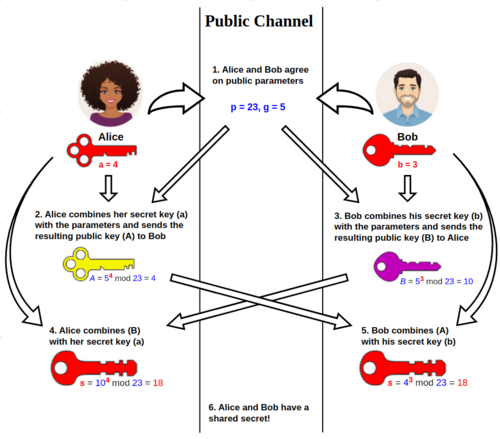
\includegraphics[scale=0.4]{DiffieHellman}

    \caption{Protokol Diffie-Hellman key exchange}
  \end{figure}
\end{frame}
\section{Matriks Komutatif Aljabar Max-Plus}
\begin{frame}
  \frametitle{\insertsection}
  \begin{definisi}[\cite{subiono2015minmaxplus}]
    Misalkan $A = (a_{ij})$ dan $B = (b_{ij})$ adalah matriks berukuran $m \times n$ dengan elemen-elemen dari $\R \cup \{\varepsilon\}$. Operasi penjumlahan dan perkalian matriks $A$ dan $B$ didefinisikan sebagai berikut:
    \begin{align*}
      (A \oplus B)_{ij}  & = a_{ij} \oplus b_{ij} = \max\{a_{ij}, b_{ij}\},                                        \\
      (A \otimes B)_{ij} & = \bigoplus_{k=1}^{n} a_{ik} \otimes b_{kj} = \max_{1 \leq k \leq n} (a_{ik} + b_{kj}).
    \end{align*}
  \end{definisi}
  {Misal:
  \[
    A = \begin{pmatrix}
      1 & 2 \\
      3 & 4
    \end{pmatrix}, \quad
    B = \begin{pmatrix}
      5 & 6 \\
      7 & 8
    \end{pmatrix},
  \]
  maka
  \[
    A \oplus B = \begin{pmatrix}
      5 & 6 \\
      7 & 8
    \end{pmatrix}, \quad
    A \otimes B = \begin{pmatrix}
      9  & 10 \\
      11 & 12
    \end{pmatrix}.
  \]}
\end{frame}
\begin{frame}
  \frametitle{\insertsection}
  \begin{definisi}[Matriks Linde-de la Puente {\cite{linde2014matricescommutinggivennormal}}]
    Untuk setiap bilangan real $r \leq 0$ dan bilangan real $k \geq 0$, kita definisikan
    \[
      [2r, r]_{n}^{k}
    \]
    sebagai himpunan matriks $A_{n\times n}$ sedemikian sehingga $a_{ii} = k$ untuk semua $i$ dan $a_{ij} \in [2r, r]$ untuk $i \neq j$.
  \end{definisi}

  \begin{teorema}[Komutativitas Matriks LdlP \cite{linde2014matricescommutinggivennormal}]
    Misalkan $A \in [2r, r]_{n}^{k_{1}}, \, B \in [2s, s]_{n}^{k_{2}}$ untuk setiap $r, s \leq 0$ dan $a_{ii} = k_{1} \geq 0, \, b_{ii} = k_{2} \geq 0$. Maka
    \[
      A \otimes B = B \otimes A = k_{2} \otimes A \oplus k_{1} \otimes B.
    \]
  \end{teorema}
\end{frame}
\section{Protokol Autentikasi Menggunakan Matriks Komutatif}
\begin{frame}
  \frametitle{\insertsection}
  Protokol Tropical Stickel Berbasis Matriks LdIP \cite{alhussaini2024implementationstickel}

  \begin{enumerate}
    \item Alice dan Bob menyepakati sebuah matriks publik $W \in \mathbb{R}_{\max}^{n \times n}$.

    \item Alice memilih dua matriks acak $A_1$ dan $A_2$, di mana $A_1 \in [2a_1, a_1]_{n}^{k_1}$ dan $A_2 \in [2a_2, a_2]_{n}^{k_2}$ sedemikian sehingga $a_1, a_2 \le 0$ dan $k_1, k_2 \ge 0$ dan mengirimkan $U = A_1 \otimes W \otimes A_2$ kepada Bob.

    \item Bob memilih dua matriks acak $B_1$ dan $B_2$, di mana $B_1 \in [2b_1, b_1]_{n}^{l_1}$ dan $B_2 \in [2b_2, b_2]_{n}^{l_2}$ sedemikian sehingga $b_1, b_2 \le 0$ dan $l_1, l_2 \ge 0$ dan mengirimkan $V = B_1 \otimes W \otimes B_2$ kepada Alice.

    \item Alice menghitung kunci rahasianya menggunakan kunci publik $V$ yang diperoleh dari Bob, yaitu $K_a = A_1 \otimes V \otimes A_2$.

    \item Bob juga menghitung kunci rahasianya menggunakan kunci publik Alice, $U$, yaitu $K_b = B_1 \otimes U \otimes B_2$.
  \end{enumerate}

\end{frame}
\begin{frame}
  \frametitle{\insertsection}
  Perhatikan bahwa
  \begin{align*}
    K_a & = A_1 \otimes V \otimes A_2                             \\
        & = A_1 \otimes (B_1 \otimes W \otimes B_2) \otimes A_2   \\
        & = (A_1 \otimes B_1) \otimes W \otimes (B_2 \otimes A_2) \\
        & = (B_1 \otimes A_1) \otimes W \
        & = B_1 \otimes (A_1 \otimes W \otimes A_2) \otimes B_2   \\
        & = B_1 \otimes U \otimes B_2 = K_b.
  \end{align*}
  Kedua pihak berakhir dengan kunci yang identik karena sifat asosiatif dan komutatif dari matriks Linde-de la Puente.

\end{frame}
\section{Contoh Permasalahan}
\begin{frame}
  \frametitle{\insertsection}
  \citeauthor{ziaulhaq2023protokol} mencotohkan sebuah permasalahan berikut:\\~\\
  Alice dan Bob mempublikasikan matriks
  \[
    W =
    \begin{pmatrix}
      30 & 24  & 26  \\
      12 & -18 & 34  \\
      34 & -21 & -20
    \end{pmatrix}
    \in \mathbb{R}_{\max}^{3 \times 3}.
  \]
  Alice memilih secara rahasia dua buah matriks
  \[
    A_1 =
    \begin{pmatrix}
      24  & -12 & -18 \\
      -24 & 24  & -15 \\
      -17 & -13 & 24
    \end{pmatrix}
    \in [-24, -12]^{24}_{3}
    \quad \text{dan} \quad
    A_2 =
    \begin{pmatrix}
      21  & -15 & -30 \\
      -18 & 21  & -22 \\
      -24 & -27 & 21
    \end{pmatrix}
    \in [-30, -15]^{21}_{3}
  \]
\end{frame}
\begin{frame}
  \frametitle{\insertsection}
  selanjutnya Alice menghitung
  \begin{align*}
    U & = A_1 \otimes W \otimes A_2 \\
      & =
    \begin{pmatrix}
      24  & -12 & -18 \\
      -24 & 24  & -15 \\
      -17 & -13 & 24
    \end{pmatrix}
    \otimes
    \begin{pmatrix}
      30 & 24  & 26  \\
      12 & -18 & 34  \\
      34 & -21 & -20
    \end{pmatrix}
    \otimes
    \begin{pmatrix}
      21  & -15 & -30 \\
      -18 & 21  & -22 \\
      -24 & -27 & 21
    \end{pmatrix}                 \\
      & =
    \begin{pmatrix}
      54 & 48 & 50 \\
      36 & 6  & 58 \\
      58 & 7  & 21
    \end{pmatrix}
    \otimes
    \begin{pmatrix}
      21  & -15 & -30 \\
      -18 & 21  & -22 \\
      -24 & -27 & 21
    \end{pmatrix}                 \\
      & =
    \begin{pmatrix}
      75 & 69 & 71 \\
      57 & 31 & 79 \\
      79 & 43 & 42
    \end{pmatrix}.
  \end{align*}
\end{frame}

\begin{frame}
  \frametitle{\insertsection}
  Selanjutnya Alice mengirimkan $U$ kepada Bob. Pada lain pihak, Bob menerima $U$. Langkah selanjutnya Bob memilih secara rahasia dua buah matriks
  \[
    B_1 =
    \begin{pmatrix}
      32  & -40 & -36 \\
      -37 & 32  & -29 \\
      -25 & -21 & 32
    \end{pmatrix}
    \in [-40, -20]^{32}_{3},
    \quad \text{dan} \quad
    B_2 =
    \begin{pmatrix}
      29  & -17 & -18 \\
      -19 & 29  & -20 \\
      -33 & -34 & 29
    \end{pmatrix}
    \in [-34, -17]^{29}_{3}.
  \]
\end{frame}

\begin{frame}
  \frametitle{\insertsection}
  Selanjutnya Bob menghitung
  \begin{align*}
    V & = B_1 \otimes W \otimes B_2 \\
      & =
    \begin{pmatrix}
      32  & -40 & -36 \\
      -37 & 32  & -29 \\
      -25 & -21 & 32
    \end{pmatrix}
    \otimes
    \begin{pmatrix}
      30 & 24  & 26  \\
      12 & -18 & 34  \\
      34 & -21 & -20
    \end{pmatrix}
    \otimes
    \begin{pmatrix}
      29  & -17 & -18 \\
      -19 & 29  & -20 \\
      -33 & -34 & 29
    \end{pmatrix}                 \\
      & =
    \begin{pmatrix}
      62 & 56 & 58 \\
      44 & 14 & 66 \\
      66 & 11 & 13
    \end{pmatrix}
    \otimes
    \begin{pmatrix}
      29  & -17 & -18 \\
      -19 & 29  & -20 \\
      -33 & -34 & 29
    \end{pmatrix}                 \\
      & =
    \begin{pmatrix}
      91 & 85 & 87 \\
      73 & 43 & 95 \\
      95 & 49 & 48
    \end{pmatrix}.
  \end{align*}
\end{frame}
\begin{frame}
  \frametitle{\insertsection}
  Setelah menghitung $V$, Bob mengirimkan tantangan tersebut kepada Alice.
  Selanjutnya Alice menerima tantangan $V$ dari Bob dan mengirimkan respon kepada Bob yaitu
  \[
    P = A_1 \otimes V \otimes A_2
  \]
  \begin{align*}
    P & =
    \begin{pmatrix}
      24  & -12 & -18 \\
      -24 & 24  & -15 \\
      -17 & -13 & 24
    \end{pmatrix}
    \otimes
    \begin{pmatrix}
      91 & 85 & 87 \\
      73 & 43 & 95 \\
      95 & 49 & 48
    \end{pmatrix}
    \otimes
    \begin{pmatrix}
      21  & -15 & -30 \\
      -18 & 21  & -22 \\
      -24 & -27 & 21
    \end{pmatrix} \\[1ex]
      & =
    \begin{pmatrix}
      115 & 109 & 111 \\
      97  & 67  & 119 \\
      119 & 73  & 82
    \end{pmatrix}
    \otimes
    \begin{pmatrix}
      21  & -15 & -30 \\
      -18 & 21  & -22 \\
      -24 & -27 & 21
    \end{pmatrix} \\[1ex]
      & =
    \begin{pmatrix}
      136 & 130 & 132 \\
      118 & 92  & 140 \\
      140 & 104 & 103
    \end{pmatrix}.
  \end{align*}
\end{frame}

\begin{frame}
  \frametitle{\insertsection}
  Bob menerima respon $P$ dari Alice. Untuk melakukan autentikasi, Bob menghitung apakah $B_1 \otimes U \otimes B_2 = P$.
  Setelah dicek ternyata
  \begin{align*}
    B_1 \otimes U \otimes B_2 & =
    \begin{pmatrix}
      32  & -40 & -36 \\
      -37 & 32  & -29 \\
      -25 & -21 & 32
    \end{pmatrix}
    \otimes
    \begin{pmatrix}
      75 & 69 & 71 \\
      57 & 31 & 79 \\
      79 & 43 & 42
    \end{pmatrix}
    \otimes
    \begin{pmatrix}
      29  & -17 & -18 \\
      -19 & 29  & -20 \\
      -33 & -34 & 29
    \end{pmatrix}               \\
                              & =
    \begin{pmatrix}
      107 & 101 & 103 \\
      89  & 63  & 111 \\
      111 & 75  & 74
    \end{pmatrix}
    \otimes
    \begin{pmatrix}
      29  & -17 & -18 \\
      -19 & 29  & -20 \\
      -33 & -34 & 29
    \end{pmatrix}               \\
                              & =
    \begin{pmatrix}
      136 & 130 & 132 \\
      118 & 92  & 140 \\
      140 & 104 & 103
    \end{pmatrix}.
  \end{align*}

  Bob memperoleh hasil bahwa $B_1 \otimes U \otimes B_2 = P$, sehingga proses autentikasi berhasil.

\end{frame}

\setbeamertemplate{frametitle continuation}{}
\setbeamercolor{frametitle}{bg=HIMAabu}
\setbeamercolor{frametitle}{fg=black}

\begin{frame}[allowframebreaks]{\Large Referensi}
  \printbibliography
\end{frame}
\end{document}